% === B03 - Experimentacion, muestreo y analisis ===
% David Alejandro Gonzalez Marquez
% dmarquez@dc.uba.ar / fokerman@gmail.com
% https://github.com/fokerman/Orga2Course

\documentclass[aspectratio=169]{beamer}
% \documentclass[handout]{beamer}

% % % Packages
\usepackage[sfdefault]{AlegreyaSans}
\usepackage{inconsolata}
\usepackage{multicol}
\usepackage{multirow}
\usepackage[spanish]{babel}
\usepackage[utf8]{inputenc}
\usepackage{enumerate}
\usepackage{color}
\usepackage{xcolor}
\usepackage[absolute,overlay]{textpos}
  \setlength{\TPHorizModule}{1mm}
  \setlength{\TPVertModule}{1mm}
\usepackage{framed}
\usepackage{mfirstuc} % para poner en mayusculas la primer letra
\usepackage{xspace} % para crear espacios en comandos 
\usepackage{pbox}
\usepackage{tikz}
\usepackage{mathabx}

% % % Beamer config
\usetheme{Pittsburgh}
\usecolortheme[rgb={1,0.48,0.0}]{structure}
\setbeamercolor{block title}{fg=white,bg=verdeuca}
\xdefinecolor{verdeuca}{rgb}{0.0,0.48,0.54}
\xdefinecolor{naranjauca}{rgb}{1,0.48,0.0}
\setbeamercolor{palette quaternary}{fg=white,bg=verdeuca}
\setbeamertemplate{title page}[default][colsep=-4bp, rounded=true] % remove title shadow
\setbeamertemplate{frametitle}[default][colsep=-2bp, shadow=false] % remove frame title shadow
\setbeamertemplate{navigation symbols}{} % remove navigation symbols
\beamertemplatenavigationsymbolsempty

% % % Colors
\definecolor{AzulClaro}{rgb}{.31,.506,.741}
\definecolor{Gris}{gray}{0.8}
\definecolor{Celeste}{rgb}{.255,.41,.884}
\definecolor{Rojo}{rgb}{1, 0, 0}
\definecolor{a}{rgb}{0.0, 0.53, 0.74}
\definecolor{r}{rgb}{0.89, 0.0, 0.13}
\definecolor{v}{rgb}{0.0, 0.5, 0.0}
\definecolor{y}{rgb}{0.0, 0.5, 0.5}
\definecolor{rojo}{HTML}{F1521B}
\definecolor{verde}{HTML}{80CD29}
\definecolor{amarillo}{HTML}{FABC09}
\definecolor{azul}{HTML}{00ADF1}

% % % Rename
\newcommand{\tab}[0]{\hspace{15pt}}

% % % Blocks
\setbeamercolor{block body}{fg=black, bg=black!10}
\setbeamercolor{block title}{fg=black, bg=black!20}
\setbeamercolor{coloredboxstuffNaranja}{fg=naranjauca,bg=black!10} %% PARA LOS BOX
\setbeamercolor{coloredboxstuffVerde}{fg=verdeuca,bg=black!10} %% PARA LOS BOX

% % % Start

\title{\Huge Experimentos}
\subtitle{Muestreo, análisis y gráficos}
      
\author{David Alejandro González Márquez}
\institute{Departamento de Computación\\
Facultad de Ciencias Exactas y Naturales\\
Universidad de Buenos Aires}
\date{}

\begin{document}

\begin{frame}
  \titlepage
\end{frame}

\begin{frame}
    \frametitle{Agenda}
    \Large
    \begin{itemize}
      \item \fbox{\texttt{1}} ¿Cómo medir tiempos?
      \vskip 15pt
      \item \fbox{\texttt{2}} ¿Cómo armar experimentos?
      \vskip 15pt
      \item \fbox{\texttt{3}} ¿Qué muestran los gráficos?
      \vskip 15pt
      \item \fbox{\texttt{4}} Ejemplos
    \end{itemize}
\end{frame}

\section{1 - ¿Cómo medir tiempos?}

\begin{frame}[fragile]
    \frametitle{ \vspace{-1cm} \flushright \colorbox{verdeuca}{ \small \textcolor{white}{ \footnotesize \secname } }\\
    ¿Qué medir?}
    \vskip -10pt
    \centering Valores muy chicos o muy grandes\\
    \vskip 5pt
    \includegraphics[scale=0.55]{img/ejemplos-layer1.pdf} \hskip 50pt 
    \includegraphics[scale=0.55]{img/ejemplos-layer2.pdf}\\
    \vskip 5pt \pause
    \centering Relación entre valores sin importar la magnitud\\
    \vskip 5pt
    \includegraphics[scale=0.55]{img/ejemplos-layer3.pdf} \hskip 50pt
    \includegraphics[scale=0.55]{img/ejemplos-layer4.pdf}\\
\end{frame}

\begin{frame}[fragile]
    \frametitle{ \vspace{-1cm} \flushright \colorbox{verdeuca}{ \small \textcolor{white}{ \footnotesize \secname } }\\
    ¿Qué medir?}
    \begin{itemize}
     \item \Large \textbf{Tiempo} \normalsize $\rightarrow$ \textcolor{naranjauca}{(numerito seguido de su unidad)}\\
     Podemos medir en unidades de tiempo, como microsegundos.
     El problema es que para eventos que suceden muy rápidamente la precisión de los relojes es insuficiente.
     \vskip 20pt \pause
     \item \Large \textbf{Ticks de Reloj} \normalsize $\rightarrow$ \textcolor{naranjauca}{(numerito sin unidad)}\\
     Para obtener el contador de ticks en Intel utilizamos la instrucción \texttt{rdtsc}.
     \vskip 20pt \pause
     \item \Large \textbf{Rendimiento} \normalsize $\rightarrow$ \textcolor{naranjauca}{(numerito en términos de procentaje)}\\
     El rendimiento se obtiene a partir de una relación entre valores. Estos deben ser comparables.
    \end{itemize}
\end{frame}

\begin{frame}[fragile]
    \frametitle{ \vspace{-1cm} \flushright \colorbox{verdeuca}{ \small \textcolor{white}{ \footnotesize \secname } }\\
    ¿Qué valores se espera obtener?}
    \begin{itemize}
     \item \Large \textbf{Tiempo} \normalsize \\
     Un número que represente un tiempo, si es muy grande entonces serán segundos, horas, días.
     Si es muy chico serán microsegundos, nanosegundos.\\
     \footnotesize \textcolor{black!50}{¿Es razonable demorar 3 segundos para ejecutar 1000 instrucciones?}
     \vskip 10pt \pause
     \item \Large \textbf{Rendimiento} \normalsize \\
     Denota la diferencia de rendimiento entre dos implementaciones. Se expresa como porcentajes.\\
     \footnotesize \textcolor{black!50}{$120\%$, puede significar que A es $20\%$ más eficiente en tiempo que B.}\\
     \footnotesize \textcolor{black!50}{$120\%$, puede significar que A demora un $20\%$ más que B.}\\
     \footnotesize \textcolor{black!50}{$10\%$, puede significar que A demora el $10\%$ de B.}
     \vskip 10pt \pause
     \item \Large \textbf{Ticks de Reloj} \normalsize \\
     Son valores enteros muy grandes. Nos va a interesar la relación entre estos.\\
     \footnotesize \textcolor{black!50}{Dos implementaciones que demoran $190231359147543$ y $192125445767335$ ticks, tienen igual rendimiento.}
    \end{itemize}
\end{frame}

\begin{frame}[fragile]
    \frametitle{ \vspace{-1cm} \flushright \colorbox{verdeuca}{ \small \textcolor{white}{ \footnotesize \secname } }\\
    ¿Qué puede afectar la medición?}
    \begin{itemize}
     \item \Large Ruido del sistema \normalsize \\
     Nuestra aplicación \textbf{no corre sola} en el sistema, la interacción con otras aplicaciones genera ruido.
     \vskip 10pt  \pause
     \item \Large Datos de entrada \normalsize \\
     Puede existir alguna \textbf{característica especial} de nuestros datos de entrada que generen una medición no esperada.
     \vskip 10pt  \pause
     \item \Large Sistema Operativo \normalsize \\
     El sistema operativo y su \textbf{accionar afecta} nuestra medición. Debemos controlarlo.
    \vskip 10pt  \pause
     \item \Large El propio procesador \normalsize \\
     Los \textbf{mecanismos de optimización} del rendimiento de un procesador afectan la medición,
     aumentando y disminuyendo la frecuencia de trabajo de las distintas partes.
    \end{itemize}
\end{frame}

\begin{frame}[fragile]
    \frametitle{ \vspace{-1cm} \flushright \colorbox{verdeuca}{ \small \textcolor{white}{ \footnotesize \secname } }\\
    ¿Cómo evitar \emph{outliers}?}
    Sean las siguientes muestras de datos,\\
    \vskip 5pt
    \small \texttt{> a = c(\textcolor{verdeuca}{32, 55, 32, 54, 65, 32, 33, 54, 78,} \textcolor{red}{2093486723}) }\\
    \small \texttt{> b = c(\textcolor{verdeuca}{32, 55, 32, 54, 65, 32, 33, 54, 78}) }\\
    \vskip 5pt \pause
    \small \texttt{> mean(a)}\\
    \small \texttt{\tab \tab \tab \tab 209348716}\\
    \small \texttt{> mean(b)}\\
    \small \texttt{\tab \tab \tab \tab 48.33333}
    \vskip 5pt
    \small \texttt{> sd(a)}\\
    \small \texttt{\tab \tab \tab \tab 662018614}\\
    \small \texttt{> sd(b)}\\
    \small \texttt{\tab \tab \tab \tab 16.9632}\\
    \vskip 5pt \pause
    Se debe poder evitar y controlar la aparición de \emph{outliers}.
    En el caso de tener \emph{outliers}, se debe poder clasificarlos y removerlos de la muestra.
    \vskip 5pt
    \textbf{Debemos armar un protocolo para realizar nuestras mediciones}
\end{frame}

\section{2 - ¿Cómo armar experimentos?}

\begin{frame}[fragile]
    \frametitle{ \vspace{-1cm} \flushright \colorbox{verdeuca}{ \small \textcolor{white}{ \footnotesize \secname } }\\
    ¿Qué analizar?}
    Debemos entender qué vamos a analizar, \small
    \begin{itemize}
     \item \textbf{Cuánto demora una implementación:}\\
     Obtener una medida de tiempo para relacionarla en un contexto
     \vskip 2pt \pause
     \item \textbf{Comparar dos implementaciones:}\\
     Obtener la diferencia de tiempos o de procentaje relativo entre dos implementaciones
     \vskip 2pt \pause
     \item \textbf{Comparar el uso de distintas instrucciones:}\\
     Obtener una medida de mejora con respecto a utilizar un determinado conjunto de instrucciones con respecto a otro
     \vskip 2pt \pause
     \item \textbf{Medir el rendimiento de una implementación:}\\
     Obtener el porcentaje de mejora de una implementación con respecto a una implementación patrón
     \vskip 2pt \pause
     \item \textbf{Factor limitante en una implementación:}\\
     Obtener una medida relativa de rendimiento con respecto a forzar un factor (ej. memoria, saltos)
     \vskip 2pt \pause
     \item \textbf{Análisis del comportamiento de una implementación:}\\
     Rendimiento bajo distinto conjunto de párametros de entrada.
    \end{itemize}
\end{frame}

\begin{frame}[fragile]
    \frametitle{ \vspace{-1cm} \flushright \colorbox{verdeuca}{ \small \textcolor{white}{ \footnotesize \secname } }\\
    ¿Qué resultado se espera?}
    \begin{itemize}
    \item \textcolor{blue!50}{A} \textbf{mantiene} su rendimiento cuando se modifican los parámetros de entrada.\pause
    \item \textcolor{blue!50}{A} \textbf{varía} su rendimiento cuando se modifican los parámetros de entrada.\pause
        \begin{itemize}
            \item Variación correlacionada con una función, predecible.
            \item No predecible, relacionada con factores externos a los parámetros de entrada.
        \end{itemize}\pause
    \item \textcolor{blue!50}{A} es \textbf{más rápido} que \textcolor{blue!50}{B}
        \begin{itemize}
            \item en tiempo
            \item en porcentaje
        \end{itemize}\pause
    \item \textcolor{blue!50}{A} se \textbf{comporta igual} a \textcolor{blue!50}{B}
        \begin{itemize}
            \item diferencia no significativa
        \end{itemize}\pause
    \item \textcolor{blue!50}{A} y \textcolor{blue!50}{B} se \textbf{comportan muy diferente}
        \begin{itemize}
            \item analizar casos independientemente
        \end{itemize}
    \end{itemize}
\end{frame}

\begin{frame}[fragile]
    \frametitle{ \vspace{-1cm} \flushright \colorbox{verdeuca}{ \small \textcolor{white}{ \footnotesize \secname } }\\
    ¿Cómo armar datos de entrada?}
    Los datos de entrada se toman de casos reales o se generan artificialmente.\\
    \vskip 10pt \pause
    Se crean,
    \begin{itemize}
     \item \normalsize \textbf{Modificando una variable}\\
     \tab \scriptsize \textcolor{black!50}{Ej. Alterando el valor de una componente de color en una imagen}
     \item \normalsize \textbf{Modificando un conjunto de variables bajo una regla}\\
     \tab \scriptsize \textcolor{black!50}{Ej. Alterando el tamaño de una imagen en ancho y alto al mismo tiempo}
    \end{itemize}
    \vskip 10pt \pause
    Tener en cuenta,
    \begin{itemize}
     \item \normalsize Variables seleccionadas
     \item \normalsize Cantidad total de entradas
     \item \normalsize Entrada común o tipo
    \end{itemize}
\end{frame}

\begin{frame}[fragile]
    \frametitle{ \vspace{-1cm} \flushright \colorbox{verdeuca}{ \small \textcolor{white}{ \footnotesize \secname } }\\
    ¿Cómo analizar resultados?}
    La etapa de discusión de los resultados, implica cuestionar las hipótesis sobre las que construimos nuestro experimento.
    \vskip 10pt
    \small
    \begin{itemize}
     \item ¿El resutado es esperado?
     \vskip 5pt
     \item ¿Existe algún factor que no estamos teniendo en consideración?
     \vskip 5pt
     \item ¿Es posible validar nuestro resultado con un experimento control?
     \vskip 5pt
     \item Si el resultado no es el esperado, ¿el experimento es incorrecto?
     \vskip 5pt
     \item Si los resultados son correctos, ¿hacer un nuevo experimento?
    \end{itemize}
\end{frame}

\section{3 - ¿Qué muestran los gráficos?}

\begin{frame}[fragile]
    \frametitle{ \vspace{-1cm} \flushright \colorbox{verdeuca}{ \small \textcolor{white}{ \footnotesize \secname } }\\
    ¿Qué se quiere mostrar?}
    Dependiendo que se quiera mostrar, se puede utilizar un tipo de gráfico u otro.
    \vskip 10pt
    \begin{itemize}
     \item \textbf{Rendimiento / Tiempo}: Area, Barras, Líneas
     \vskip 10pt
     \item \textbf{Relaciones}: Líneas, Dispersión
     \vskip 10pt
     \item \textbf{Porcentajes}: Torta, Area o Barras acumuladas
     \vskip 10pt
     \item \textbf{Comportamiento / Variación}: Líneas, Superficie
    \end{itemize}
\end{frame}

\begin{frame}[fragile]
    \frametitle{ \vspace{-1cm} \flushright \colorbox{verdeuca}{ \small \textcolor{white}{ \footnotesize \secname } }\\
    ¿Qué colores? ¿Qué tipo de gráfico? ¿Qué escala?}
    \textbf{Colores}
     \begin{itemize}
      \item Gusto / estética
      \item Resaltar un dato sobre otro
      \item Pensar en el medio de distribución (impreso)
     \end{itemize}
    \vskip 10pt
    \textbf{Tipo}
     \begin{itemize}
      \item El que mejor muestre la información (ojo con 3d)
      \item Que sirva para explicar (sin información de más)
     \end{itemize}
     \vskip 10pt
    \textbf{Escala}
     \begin{itemize}
      \item Lineal o Logarítmica
      \item Sobre qué eje va cada escala
      \item Valores en los ejes
     \end{itemize}
\end{frame}

\section{4 - Ejemplos}

\begin{frame}[fragile]
    \frametitle{ \vspace{-1cm} \flushright \colorbox{verdeuca}{ \small \textcolor{white}{ \footnotesize \secname } }\\
    Humor de XKCD}
    \begin{textblock}{500}(40,12)  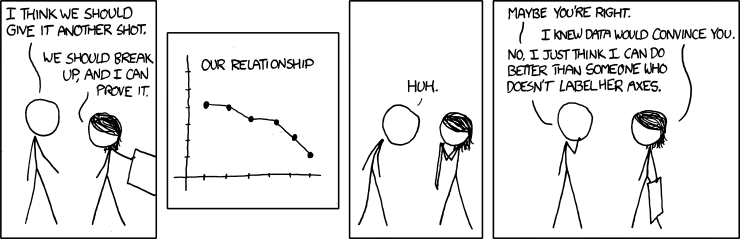
\includegraphics[scale=0.40]{img/convincing_en.png} \end{textblock}
    \begin{textblock}{500}(40,50) 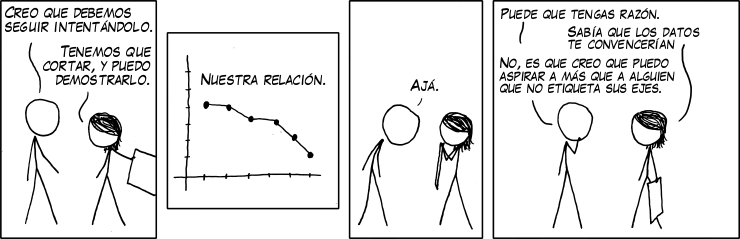
\includegraphics[scale=0.40]{img/convincing_es.png} \end{textblock}
\end{frame}

\begin{frame}[fragile,t]
    \frametitle{ \vspace{-1cm} \flushright \colorbox{verdeuca}{ \small \textcolor{white}{ \footnotesize \secname } }\\
    Ejemplo 1: Comparando datos}
    No podemos agrupar en un gráfico cosas que no tiene nada que ver entre ellas.
    \begin{textblock}{500}(1,25)  \only<1->{\includegraphics[scale=0.5]{img/fig1A.pdf}} \end{textblock}
    \begin{textblock}{500}(78,25) \only<2->{\includegraphics[scale=0.5]{img/fig1B.pdf}} \end{textblock}
    \begin{textblock}{500}(78,25) \only<3->{\includegraphics[scale=0.5]{img/fig1C.pdf}} \end{textblock}
    \begin{textblock}{500}(11,27) \only<2->{\textcolor{rojo}{\textbf{MAL}}}   \end{textblock}
    \begin{textblock}{500}(88,27) \only<2->{\textcolor{verde}{\textbf{BIEN}}} \end{textblock}
\end{frame}

\begin{frame}[fragile,t]
    \frametitle{ \vspace{-1cm} \flushright \colorbox{verdeuca}{ \small \textcolor{white}{ \footnotesize \secname } }\\
    Ejemplo 2: Analizando límites, tendencias o comportamientos anómalos}
    Escalas: Podemos setear la escala de cada eje con distintos criterios (lineal, log, loglog, etc).
    \begin{textblock}{500}(1,25)  \only<1->{\includegraphics[scale=0.45]{img/fig2A.pdf}} \end{textblock}
    \begin{textblock}{500}(78,25) \only<2->{\includegraphics[scale=0.45]{img/fig2B.pdf}} \end{textblock}
    \begin{textblock}{500}(11,27) \only<2->{\textcolor{rojo}{\textbf{MAL}}}   \end{textblock}
    \begin{textblock}{500}(88,27) \only<2->{\textcolor{verde}{\textbf{BIEN}}} \end{textblock}
    \begin{textblock}{500}(90,83) \only<2->{\textbf{Cambiamos el eje y a escala logarítmica}} \end{textblock}
\end{frame}

\begin{frame}[fragile,t]
    \frametitle{ \vspace{-1cm} \flushright \colorbox{verdeuca}{ \small \textcolor{white}{ \footnotesize \secname } }\\
    Ejemplo 3: Proporciones}
    Un gráfico de torta sirve para  ver proporciones en un TODO. \\ \textcolor{rojo}{No! para agrupar valores que no constituyen un todo.}
    \begin{textblock}{500}(-1,30) \only<2->{\includegraphics[scale=0.5]{img/fig3A.pdf}} \end{textblock}
    \begin{textblock}{500}(78,28) \only<3->{\includegraphics[scale=0.45]{img/fig3B.pdf}} \end{textblock}
    \begin{textblock}{500}(11,29) \only<3->{\textcolor{rojo}{\textbf{MAL}}}   \end{textblock}
    \begin{textblock}{500}(86,29) \only<3->{\textcolor{verde}{\textbf{BIEN}}} \end{textblock}
    \begin{textblock}{500}(90,83) \only<3->{\textbf{Barras es la opción}} \end{textblock}
\end{frame}

\begin{frame}[fragile,t]
    \frametitle{ \vspace{-1cm} \flushright \colorbox{verdeuca}{ \small \textcolor{white}{ \footnotesize \secname } }\\
    Ejemplo 4: Optimizar un parámetro}
    Tenemos que encontrar el parámetro óptimo.\\
    \begin{textblock}{500}( 6,26) \only<2->{\includegraphics[scale=0.45]{img/fig4A.pdf}} \end{textblock}
    \begin{textblock}{500}(14,26) \only<3->{\textcolor{rojo}{\textbf{MAL}}}   \end{textblock}
    \begin{textblock}{500}(12,83) \only<3-3>{\textbf{No conocemos el error de nuestros datos}} \end{textblock}
    \begin{textblock}{500}(12,83) \only<4->{\textbf{Utilizamos barras de error}} \end{textblock}
    \begin{textblock}{500}(78,26) \only<4-5>{\includegraphics[scale=0.45]{img/fig4B.pdf}} \end{textblock}
    \begin{textblock}{500}(86,26) \only<5-5>{\textcolor{rojo}{\textbf{MAL}}} \end{textblock}
    \begin{textblock}{500}(90,83) \only<5-5>{\textbf{Los errores NO están acotados}} \end{textblock}
    \begin{textblock}{500}(78,26) \only<6->{\includegraphics[scale=0.45]{img/fig4C.pdf}} \end{textblock}
    \begin{textblock}{500}(86,26) \only<6->{\textcolor{verde}{\textbf{BIEN}}} \end{textblock}
    \begin{textblock}{500}(90,83) \only<6->{\textbf{Los errores están acotados}} \end{textblock}
\end{frame}

\begin{frame}[fragile,t]
    \frametitle{ \vspace{-1cm} \flushright \colorbox{verdeuca}{ \small \textcolor{white}{ \footnotesize \secname } }\\
    Ejemplo 5: Analizando límites}
    \vskip 5pt
    Queremos ver donde la performance varía.
    \begin{textblock}{500}(1,27)  \only<1->{\includegraphics[scale=0.45]{img/fig5A.pdf}} \end{textblock}
    \begin{textblock}{500}(78,27) \only<2->{\includegraphics[scale=0.45]{img/fig5B.pdf}} \end{textblock}
    \begin{textblock}{500}(11,27) \only<2->{\textcolor{rojo}{\textbf{MAL}}}   \end{textblock}
    \begin{textblock}{500}(88,27) \only<2->{\textcolor{verde}{\textbf{BIEN}}} \end{textblock}
    \begin{textblock}{500}(96,83) \only<2->{\textbf{Normalizamos los datos}} \end{textblock}
\end{frame}

\section{Consejos}

\begin{frame}[fragile]
    \frametitle{ \vspace{-1cm} \flushright \colorbox{verdeuca}{ \small \textcolor{white}{ \footnotesize \secname } }\\
    Pequeños pero no menos importantes consejos}
    \small
    \begin{itemize}
     \item Los resultados deben ser \textbf{reproducibles y consistentes}
     \vskip 15pt \pause
     \item Ser \textbf{ordenado en las explicaciones}, explicar tanto el código como los experimentos, datos y resultados
     \vskip 15pt \pause
     \item \textbf{No adjuntar gráficos de más}, sólo deben ir los que hagan falta
     \vskip 15pt \pause
     \item El promedio de una muestra debe estar \textbf{acompañado de su desvío}
     \vskip 15pt \pause
     \item No todo se puede explicar, existen comportamientos \textbf{inexplicables}
     \vskip 15pt \pause
     \item El informe debe ser un \textbf{trabajo integral}, consistente y bien escrito
    \end{itemize}
\end{frame}

\begin{frame}[fragile]
    \frametitle{ \vspace{-1cm} \flushright \colorbox{verdeuca}{ \small \textcolor{white}{ \footnotesize \secname } }\\
    Informe}
    \begin{textblock}{500}(30,3)
        \scriptsize %\small
        \begin{enumerate}
        \item \textbf{Implementación}
        \begin{itemize} \scriptsize
        \item Explicación general de la solución
        \item Detalles de implementación
        \item Uso de constantes y memoria
        \end{itemize}
        \item \textbf{Análisis preeliminar}
        \begin{itemize} \scriptsize
        \item Comparación de rendimiento de ASM vs C
        \item Comparar para distintos tamaños, relaciones entre implementaciones
        \end{itemize}
        \item \textbf{Hipótesis de trabajo}
        \begin{itemize} \scriptsize
        \item Conjunto de ideas de experimentos
        \item Afirmaciones que buscan probar verdaderas
        \item Deben ser concisas y claras
        \end{itemize}
        \item \textbf{Diseño experimental}
        \begin{itemize} \scriptsize
        \item Explicación de como y que van a medir
        \item Explicación del conjunto de datos de entrada
        \item Detalles de la plataforma y la configuración de la misma
        \end{itemize}
        \item \textbf{Resultados y Análisis}
        \begin{itemize} \scriptsize
        \item Resultados obtenidos, gráficos y tablas
        \item Explicación e interpretación de los resultados obtenidos
        \end{itemize}
        \item \textbf{Conclusiones}
        \begin{itemize} \scriptsize
        \item Relación entre las hipótesis de trabajo y resultados
        \end{itemize}
        \end{enumerate}
    \end{textblock}
\end{frame}

\begin{frame}[fragile]
    \frametitle{Bibliografía: Fuentes y material adicional}
    \begin{itemize}
    \item Convenciones de llamados a función en x86: \\
    \url{https://en.wikipedia.org/wiki/X86_calling_conventions}
    \item Notas sobre System V ABI: \\
    \url{https://wiki.osdev.org/System_V_ABI}
    \item Documentación de NASM: \\
    \url{https://nasm.us/doc/}
    \item Artículo sobre el flag \texttt{-pie}: \\
    \url{https://eklitzke.org/position-independent-executables}
    \item Documentación de System V ABI: \\
    \url{https://uclibc.org/docs/psABI-x86_64.pdf}
    \item Manuales de Intel: \\
    \url{https://software.intel.com/en-us/articles/intel-sdm}
    \end{itemize}
\end{frame}

\begin{frame}[plain]
\begin{center}
\vspace{2cm}
\huge ¡Gracias!\\
\vspace{2cm}
\normalsize Recuerden leer los comentarios al final de \\ este video por aclaraciones o fe de erratas.
\end{center}
\end{frame}

\end{document}
